% Use only LaTeX2e, calling the article.cls class and 12-point type.

\documentclass[12pt]{article}

%no step between enumirations
\usepackage{enumitem}

% Users of the {thebibliography} environment or BibTeX should use the
% scicite.sty package, downloadable from *Science* at
% www.sciencemag.org/about/authors/prep/TeX_help/ .
% This package should properly format in-text
% reference calls and reference-list numbers.

\usepackage{scicite}

% Use times if you have the font installed; otherwise, comment out the
% following line.

\usepackage{times}

% The preamble here sets up a lot of new/revised commands and
% environments.  It's annoying, but please do *not* try to strip these
% out into a separate .sty file (which could lead to the loss of some
% information when we convert the file to other formats).  Instead, keep
% them in the preamble of your main LaTeX source file.


% The following parameters seem to provide a reasonable page setup.

\topmargin 0.0cm
\oddsidemargin 0.2cm
\textwidth 16cm 
\textheight 21cm
\footskip 1.0cm


%The next command sets up an environment for the abstract to your paper.

\newenvironment{sciabstract}{%
\begin{quote} \bf}
{\end{quote}}


% If your reference list includes text notes as well as references,
% include the following line; otherwise, comment it out.

\renewcommand\refname{References and Notes}

% The following lines set up an environment for the last note in the
% reference list, which commonly includes acknowledgments of funding,
% help, etc.  It's intended for users of BibTeX or the {thebibliography}
% environment.  Users who are hand-coding their references at the end
% using a list environment such as {enumerate} can simply add another
% item at the end, and it will be numbered automatically.

\newcounter{lastnote}
\newenvironment{scilastnote}{%
\setcounter{lastnote}{\value{enumiv}}%
\addtocounter{lastnote}{+1}%
\begin{list}%
{\arabic{lastnote}.}
{\setlength{\leftmargin}{.22in}}
{\setlength{\labelsep}{.5em}}}
{\end{list}}

\usepackage{graphicx}
\usepackage{multirow}
\usepackage{caption}
\usepackage{subcaption}
\graphicspath{ {Diagrams/} }

% Include your paper's title here

\title{Prioritized Foraging using Robot Swarms} 


% Place the author information here.  Please hand-code the contact
% information and notecalls; do *not* use \footnote commands.  Let the
% author contact information appear immediately below the author names
% as shown.  We would also prefer that you don't change the type-size
% settings shown here.

\author
{Nicolaas J. Taljaard and Andries P. Engelbrecht\\
\\
\normalsize{Department of Computer Science, University of Pretoria, South Africa}\\
}

% Include the date command, but leave its argument blank.

\date{}



%%%%%%%%%%%%%%%%% END OF PREAMBLE %%%%%%%%%%%%%%%%



\begin{document} 

% Double-space the manuscript.

\baselineskip24pt

% Make the title.

\maketitle 



% Place your abstract within the special {sciabstract} environment.

\begin{sciabstract}
  This empirical study aims to improve on the prioritized foraging problem through using robotic swarms. The attempt will be introducing clustering before the foraging process. It focuses on swarm intelligence in cooperation with swarm robotics with social insect behaviors as the working force. Previous works shows foraging using a honey-bee approach is most successful in the dynamic environments used. The ant cluster is chosen for no in communication or pheromones are required. It was found that cluster beforehand has potential although it comes at a significantly higher iteration cost.
\end{sciabstract}


% In setting up this template for *Science* papers, we've used both
% the \section* command and the \paragraph* command for topical
% divisions.  Which you use will of course depend on the type of paper
% you're writing.  Review Articles tend to have displayed headings, for
% which \section* is more appropriate; Research Articles, when they have
% formal topical divisions at all, tend to signal them with bold text
% that runs into the paragraph, for which \paragraph* is the right
% choice.  Either way, use the asterisk (*) modifier, as shown, to
% suppress numbering.

\section{Introduction}

\par{Swarm Robotics is an entity constructed of simple behavior  robots in collaboration, the inspiration for these robot algorithms draw from social insects such as: Bees, ants and termites [Robots-Dorigo]. These insects are reliant on water, food and organization as a source of survival through search, retrieval and sorting. The described processes are the basis of the algorithms in the form of foraging and clustering [Proposal 6].}

\par{This is ideal for the mining industry for ore retrieval with shorting waiting times between blasting through the robotic abilities [Jade]. Honey bees have to explore away from their hive to search and retrieve of resources as the foraging [Proposal 11]. Also clustering which is modeled after how ant organize their dead dependent on the density of corpses locations [Proposal 8]. In mining this will improve efficiency of extracting the gold from out the mines with obstructions and rubble [Jade].} 

\par{Foraging is commonly used as a benchmark tool due to its complex and for the social level coordination required [Winfield]. As by Lumer, the ant clustering algorithm has been used to solve problems in fields such as cryptography, sorting and graphs [Lumer]. Prioritization foraging as tested by Jade [Jade] has found that the honey bee proves to be more successful in foraging in dynamic environments. This paper introduces clustering before the foraging process to way it effects on the foraging success rate, productivity and increased time requirement.}

\section{Background}

The following selections introduces further information on the field and also the clustering and foraging algorithms that are experimented with.

\subsection{Swarm Intelligence / Robotics}

\par{Swarm Intelligence (SI) as a method of problem solving through the use of agents interacting with their environment as the source of their knowledge [Beni-Robot]. The agents are represented as robots in a collective body known as Swarm Robotics. As collective intelligence of the swarm it raises the social behavior an individual robot, the test algorithms used are independent of an controlling entity to provide guidance to other robots. The independence of this allows robots to base decision on their immediate environment, their current robotic status and ability.}

\par{Swarm-based robotics (SR) is defined by Bonabeau \textit{et al} [Robot-Swarm] that it may be able to perform tasks without needing a explicit representation of the environment. These robots are modeled after insect colonies respectively as desert ants for clustering and honey bees for foraging. Each colony has their own internal communication method to achieving their goals and enable the process that is mimicked on the robots.}

\par{SI and SR as a self-organized social insects use a communication method call stigmergy [Robot-Swarm], it can be in a form of sematectonic and sign-based communication. Where sign-based is in the form of physical information exchange and sematectonic by means of environment changes. Stigmergy will be used as follow: Direct where the honey bee broadcasts a foraging site by dancing when it arrives at the hive. Also by in-direct for ant cemetery clustering where each ant exams the environment to affect its decision making.}

\subsection{Desert-ant Cemetery Clustering}

\par{The desert ant is used to model the ant clustering process, it is chosen for these ants are independent of any direct communication or information sharing. Desert ants do not require any pheromones or beacons to provide navigation it only uses vision of its immediate environment [12 Jade]. The cemetery cluster is based on the ant that move there died into clusters dependent on the observed environment and the density of object clusters [77 AI].}

\par{As for movement decisions it uses random navigation or if detection movement is towards the lowest density [13 Jade]. Once an object is picked up it is carries towards the highest dens array until it satisfies the dropping probability where it is then dropped.  This clustering process will aim at improving the performance of foraging due to the closer group of the same priority objects. The abilities of a desert ant is simplistic and does not require many detectors to be added to the robot making it viable and can be cost effective as only a camera is required.}

\subsection{Honey-bee Foraging}

\par{The honey-bee is proven by Jade [Jade] to be success foraging algorithm when working with a wider variety of grid configurations and object placing. These bees have three roles assigned to them [Jade 7]: Employed-, unemployed foragers and scouts. Scouts search the environments, once an object successfully foraged depending on its desirability it can dance for the unemployed bees. These bees wait for a dance and employed bees are actively foraging a location. As suggested by Jasen [Jade 14] waiting bees change to scout after a duration of time. An improvement made is during employed foraging, if a higher dens location is detected while following the determined Path Integration (PI) it would rather forage that  location. PI is the process where a bee continuously changes its baring vector towards its starting location to be able to share the direction other bees during the dance [Jade 22].}

\subsection{Prioritized Clustering / Foraging}

\par{An environment containing prioritized and non-prioritized object throughout may introduce the following: It may occur that prioritized items are encircled or obstructed by non-prioritized objects. There are two methods to resolve this, by foraging the non-prioritized objects or by cluster the which will separate the object types away from one another. To achieve success and optimal result for the multi-problem both of these solutions is used.}

\section{Algorithm Description}

\subsection{Desert-ant cemetery clustering}

\par{The ant cemetery clustering algorithm is dependent on the densities of an ants immediate area. A laden ant will  drop its payload if the density surpasses the probability barrier. During the scouting process ants will move towards the lowest dens area and the highest during clustering. The process and states are described by Figure.1 as follows:}
\\
\begin{figure}[h]
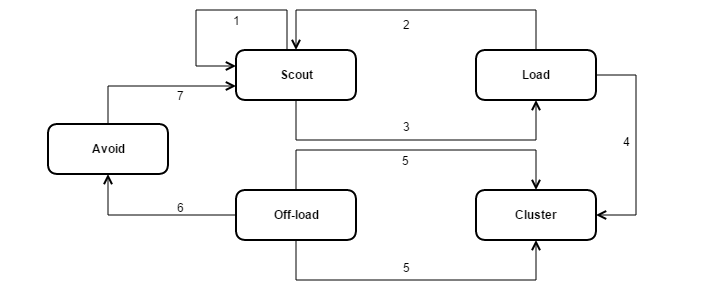
\includegraphics[width=\textwidth]{desertant.png}
\centering
\caption{Desert Ant Cemetery Clustering State Diagram}
\label{fig:desertamtState}
\end{figure}

\begin{enumerate}[nolistsep]
\item A scout searches randomly until a populated area is detected. Upon object detection scouts move towards the lowest dens area populated with objects.
\item An ant will attempt pick-up of an object once arrived at the source area. The pick-up probability is calculated with the density detected from the surrounding objects. If the probability surpasses $\phi$ it will be picked up.
\item Otherwise it will continue to follow the density and attempts to find an object that has a low enough density around it.
\item Once laden an ant changes its detection for the most dens area within its perceived vicinity.
\item The same probability calculation is used by scouting, the object will be dropped when it is above $\mu$ for successful clustering.
\item After the drop ants avoid the area for the max of its detection range, to avoid the possibility of being caught optimizing a single cluster instead of clustering outliers.
\item Finally ants resorts to the default scout method.
\end{enumerate}

\subsection{Honey-bee Foraging}

\par{The honey bee algorithm consists of two type of robots and initialized by random as unemployed foragers or scouts. The position of each robot is initialized along the starting column of the grid for an increased spread of robots. A sink where objects are drop is not limited to a single location for all robots but the initialization position of the specific robot is its own drop point. All robots states are depicted in Figure.2 and described as follows:}

\begin{figure}[h]
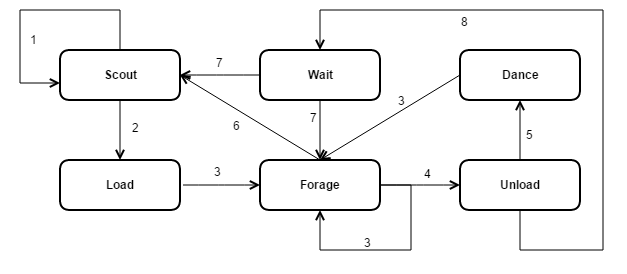
\includegraphics[width=\textwidth]{honeybee.png}
\centering
\caption{Honey Bee Foraging State Diagram}
\label{fig:honeyBeeState}
\end{figure}

\begin{enumerate}[nolistsep]
	\item A bee in the scouting state does a random walk through the environment looking for the area with it highest density of objects.
	\item Once a dens area is detected and the probability  of pick-up is greater than $\phi$ an object will be loaded and the bee will start foraging.
	\item As laden the bee forages the object along its PI back to the drop sink where it will drop the object. If not laden the bee follows the direction vector back towards the previous found location for the measured distance. During the return process a higher dens area may be detected where upon the bee will changes its bearing vector, this is done if the density is greater than 1.4 of the previous determined density.
	\item An object is unloaded from a laden bee once it reaches its sink and deposits it. If the bee was in the waiting state before foraging it will return to wait else as an unemployed forager it will continue to forage the site.
	\item After a successful deposit the bee calculates the probability of if the found site is successful. If so it will perform a dance for bee in a close vicinity to promote the sites PI as well as it distance otherwise the robot will do a solo forage.
	\item An employed forager may abort after no object where able to be found where upon it will return to the sink and go into a waiting state.
	\item A bee in the waiting state will be employed until it detects a dance within its vicinity that is deems profitable.  The bee may also resort to unemployed scouting if it does not detect a dance for a prolonged time $tmax$.
	\item A bee that was in a waiting state before being an employed forager will return a waiting state once it off-loads.
\end{enumerate}

\section{Simulation Configuration}

\par{The simulated environment is representation with a 2D grid which has values assigned for every state for robots and the type of object and their own state of carried. Each object and robot fills one index of the grid. Objects can be picked up by robots once on top of an object or move around it as an obstacle to get to higher dens areas. Where an area is calculated over a 5 index range around the robots position.}

\par{An object is successfully foraged once it reaches the end of the environment at column zero where object will be dropped and removed from the environment. The adoption to the setup for a mining environment where the sinks will be place at specific locations would be simple. Different environment layouts are used for testing, with this four object distributions: Uniform (Fig 3.a), Clustered with Lumer-Faieta (Fig 3.b), Vein (Fig 3.c), Gaussian (Fig 3.d).}
\\
\begin{figure}[h]
\centering
\begin{subfigure}{0.2\textwidth}
  \centering
  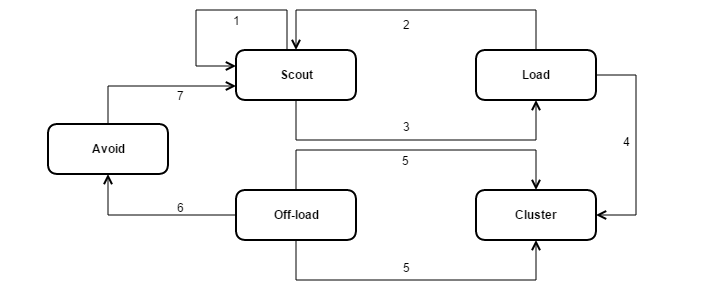
\includegraphics[width=.2\linewidth]{desertant.png}
  \caption{Uniform}
  \label{fig:sub1}
\end{subfigure}%
\begin{subfigure}{.2\textwidth}
  \centering
  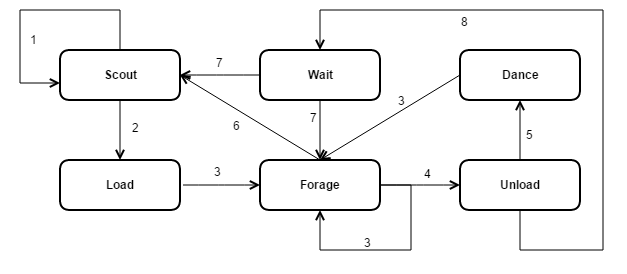
\includegraphics[width=.2\linewidth]{honeybee.png}
  \caption{Clustered}
  \label{fig:sub2}
\end{subfigure}
\begin{subfigure}{.2\textwidth}
  \centering
  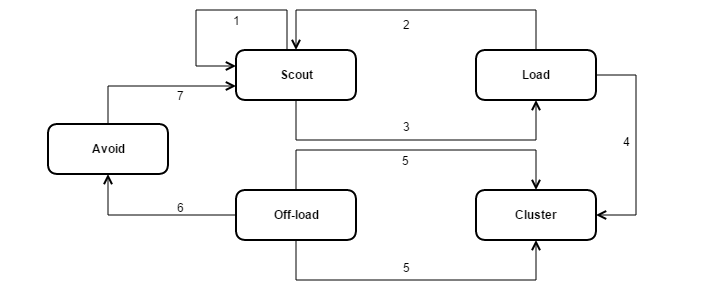
\includegraphics[width=.2\linewidth]{desertant.png}
  \caption{A Vein}
  \label{fig:sub3}
\end{subfigure}%
\begin{subfigure}{.2\textwidth}
  \centering
  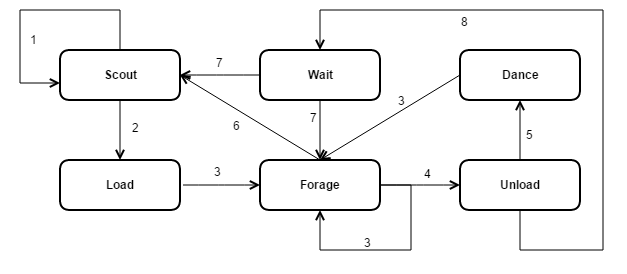
\includegraphics[width=.2\linewidth]{honeybee.png}
  \caption{Gaussian}
  \label{fig:sub4}
\end{subfigure}
\caption{Environment Scatters}
\label{fig:EnvironmentScaters}
\end{figure}

\vspace{0.3cm}

\par{The configuration are setup as follows where each is configuration is simulated 30 times. Scatter layout, the placement of object as names above to test different dispersion resulting from an explosions. Grid sizes representing the number of position units increasing complexity and required simulation time, $S = 50, 100, 200$. The amount of robots used to cluster and forage objects, $c = 10, 30, 50, 70, 100$. Grid coverage as a percentage of objects placed against open locations for movement, $p = 5\%, 20\%, 50\%, 70\%, 90\%$. A ratio representation, $r = 0.2, 0.25, 0.333, 0.5, 0.667, 0.75, 0.8, 1$ as the number of prioritized objects against non-prioritized object. A priority value is used to determine the priority of a populated area calculated per item detected for $\tau = 0.2, 0.25, 0.333, 0.5, 0.667, 0.75, 0.8, 1$. Honey-bee specific values are used for the allowed waiting time of $tmax = 100$, the max time spent foraging is determine by $1.3$ times of the distance acquired from the dance.}

\par{A stagnation condition has been created to prevent endless random walks that is determined from when the last pick up occurred. This stagnation limit is set at $400$ time the grid size which is applied to the clustering and foraging processes. Also a $100 000$ limit on iterations across both pre-clustering is required and foraging combined.}

\section{Results}

The result will use the priority of item, ratio of items and the iteration count aimed at solving the following hypotheses with regards to the percentage of items foraged: 
\begin{enumerate}[nolistsep]
	\item The relative effect of stagnation and set limitation across the algorithms.
	\item Pre-clustering will increase the success rate that more priority items are foraged against only performing foraging.
	\item Pre-clustering will require a higher iteration count but will be acceptable due to a significantly higher success rate.
\end{enumerate}
Section 5.1 to 5.3 will cover each hypotheses independently, attempting to solve each through statistical results of the simulation of above. 

\subsection{Relation between Performance and Stopping Conditions}

\par{This section aim to establish the time impact that pre-clustering has the process against only foraging. Due to the constraint on stagnation as well as iteration count causes that an amount of simulation are preemptively stopped. As from the percentages of stopped simulations shown in Table 5:}
\\
\begin{table}[h]
\centering
\begin{tabular}{|l|l|l|l|}
\hline
            & Stagnated & Limited & Average Iterations \\ \hline
Non-Cluster & 20.95     & 0.0     & 36073              \\ \hline
Pre-Cluster & 31.06     & 35.5    & 77578              \\ \hline
\end{tabular}
\caption{Stopping Condition Limitations as Percentages}
\label{my-label}
\end{table}

\par{These statistics are recorded over the entire simulation, including the pre-clustering process when it is used. This indicates that the clustering consumes a high amount of iteration from the $2.15$ increase on iteration count.}

\par{The stagnation rate is based on the amount of iterations robots spend unladen, it is preemptively stopped once the above set limit is passed. As these statistics show $66.56\%$ of the the pre-cluster simulations where preemptively stopped where only $20.95\%$ of non-cluster was affected. Although this has hindered the performance of the simulations it has still performed exceptionally.}

\subsection{Relation between Item Priority and Ratio of Items Analysis with Regards to Foraging Success}
\par{The relation analysis of $r$ and $\tau$ is describe in Table 2 as a representation of how successful the simulations where. These values were calculated in terms of the percentage of items foraged against the amount of priority items placed. A condensate form is shown in Table 1.}
\\
\begin{table}[h]
\centering
\begin{tabular}{|l|l|l|}
\hline
            & Average & Std Dev \\ \hline
Non-Cluster & 0.884   & 0.279   \\ \hline
Pre-Cluster & 0.740   & 0.361   \\ \hline
\end{tabular}
\caption{Performance Summation}
\label{my-label}
\end{table}

\par{As from shown the pre-cluster as been slightly less successful then the Honey Bee foraging alone. Although the pre-clustering has still obtained a higher success rate for dynamic environments as tested by Jade [Jade]. Also improvements made on the implementation [Jade] has shown a $7.7\%$ increase on success rate and also a $1.5\%$ lower standard deviation for the Honey-Bee foraging without clustering. The detailed overview of the analysis is giving in Table 3. }

\begin{table}[h]
\centering
\begin{tabular}{|l|l|l|l|l|l|l|l|l|l|}
\hline
\multirow{2}{*}{Algorithm}                         & \multirow{2}{*}{\hspace{0.017\linewidth}$r$} & \multicolumn{8}{l|}{\hspace{0.28\linewidth} $t$}                                                                                        \\ \cline{3-10} 
                                                   &                    & 0.2         & 0.25        & 0.33        & 0.5         & 0.667       & 0.75        & 0.8         & 1.0         \\ \hline
\multirow{8}{*}{Non-Cluster}                       & 0.2                & 0.700       & 0.540       & 0.898       & 0.799       & {\bf 0.968} & 0.893       & {\bf 0.941} & {\bf 0.998} \\
                                                   & 0.25               & {\bf 0.999} & {\bf 0.999} & {\bf 1.000}   & {\bf 1.000}   & 0.968       & {\bf 1.000}   & {\bf 0.950}       & 0.697       \\
                                                   & 0.33               & 0.554       & 0.899       & 0.819       & {\bf 0.961} & {\bf 0.904} & {\bf 0.938} & {\bf 0.901} & 0.561       \\
                                                   & 0.5                & 0.792       & 0.712       & {\bf 0.954}       & 0.885       & {\bf 0.992} & {\bf 0.941} & {\bf 0.994} & {\bf 1.000}   \\
                                                   & 0.667              & {\bf 1.000}   & {\bf 1.000}   & {\bf 1.000}   & {\bf 0.968} & {\bf 0.950} & 0.900       & 0.576       & 0.800       \\
                                                   & 0.75               & 0.730       & {\bf 0.951} & 0.894       & {\bf 0.995} & {\bf 0.939} & 0.706       & 0.571       & 0.895       \\
                                                   & 0.8                & 0.826       & {\bf 0.975} & 0.893       & 0.942       & {\bf 0.999} & {\bf 0.999} & {\bf 1.000}   & {\bf 1.000}   \\
                                                   & 1.0                & {\bf 1.000}   & {\bf 0.968} & {\bf 1.00}   & {\bf 0.950} & 0.717       & 0.561       & {\bf 0.900}       & 0.810       \\ \hline
\multirow{8}{*}{\begin{tabular}[c]{@{}c@{}} Pre-Cluster\end{tabular}} & 0.2                & 0.690       & 0.488       & {\bf 0.890} & 0.690       & \bf{0.960}       & 0.680       & {\bf 0.890} & 0.756                 \\
                                                                               & 0.25               & 0.870       & {\bf 0.995} & 0.722       & \bf{0.914}       & 0.632       & {\bf 0.948} & 0.564       & 0.716                 \\
                                                                               & 0.33               & 0.528       & {\bf 0.899} & 0.684       & {\bf 0.814} & 0.466       & 0.448       & 0.469       & 0.542                \\
                                                                               & 0.5                & 0.756       & 0.638       & {\bf 0.906} & 0.710       & {\bf 0.968} & 0.652       & {\bf 0.998} & 0.869                 \\
                                                                               & 0.667              & {\bf 1.000} & 0.637       & {\bf 1.000} & 0.579       & 0.884       & 0.590       & 0.574       & 0.762               \\
                                                                               & 0.75               & 0.674       & {\bf 0.837} & 0.656       & 0.503       & 0.284       & 0.706       & 0.506       & {\bf 0.898}                 \\
                                                                               & 0.8                & 0.695       & {\bf 0.956} & 0.682       & {\bf 0.890} & 0.756       & {\bf 0.876} & {\bf 0.997} & 0.723                 \\
                                                                               & 1.0                  & {\bf 0.916} & 0.632       & {\bf 0.947} & 0.564       & 0.731       & 0.534       & {\bf 0.905}       & 0.716                 \\ \hline
\end{tabular}
\caption{Completion Based Performance}
\label{my-label}
\end{table}

\par{The pre-clustering algorithm has high success points but also due to the limitations discussed above low point creep in. This how ever does not hinder the performance showing pre-clustering does in fact show promise and the ability to increase the overall success rate of the foraging process.}

\subsection{Relation between Item Priority and Ratio of Items Analysis with Regards to Duration}

\par{This section uses the amount of iterations against the success rate achieved during the simulation. The higher the success rate the lower the shown value and the inverse is the true for the iteration count. Table 4 shows a summation of the process time verses its success rates.}
\\
\begin{table}[h]
\centering
\begin{tabular}{|l|l|l|}
\hline
            & Average & Std Dev \\ \hline
Non-Cluster & 0.042   & 0.421   \\ \hline
Pre-Cluster & 0.268   & 0.311   \\ \hline
\end{tabular}
\caption{Time-Performance Summation}
\label{my-label}
\end{table}

\par{As Table 4 shows the pre-clustering is a not every efficient regarding item foraging per iteration. It proves to have be $6$ times less efficient per iteration then only foraging with regards to time constraints. Although it has a lower standard deviation resulting in a more consistent result. This may be due to the high amount of simulations being limited by iterations.}
\\
\begin{table}[h]
\centering
\begin{tabular}{|l|l|l|l|l|l|l|l|l|l|}
\hline
\multirow{2}{*}{Algorithm}                         & \multirow{2}{*}{\hspace{0.017\linewidth}$r$} & \multicolumn{8}{l|}{\hspace{0.28\linewidth} $t$}                                                                                         \\ \cline{3-10} 
                                                   &                    & 0.2         & 0.25        & 0.33         & 0.5         & 0.667       & 0.75        & 0.8         & 1.0         \\ \hline
\multirow{8}{*}{Non-Cluster}                       & 0.2                & {\bf 0.057} & 0.180       & {\bf 0.0567} & 0.338       & 0.146       & 0.454       & 0.325       & 0.500       \\
                                                   & 0.25               & 0.253       & {\bf 0.123} & 0.492        & 0.177       & 0.563       & 0.180       & 0.672       & {\bf 0.052} \\
                                                   & 0.33               & 0.190       & {\bf 0.081} & 0.422        & 0.140       & 0.544       & 0.326       & 0.504       & {\bf 0.065} \\
                                                   & 0.5                & 0.166       & 0.253       & 0.192        & 0.440       & 0.208       & 0.632       & {\bf 0.073} & 0.286       \\
                                                   & 0.667              & {\bf 0.102} & 0.522       & 0.142        & 0.564       & 0.308       & 0.482       & {\bf 0.066} & 0.170       \\
                                                   & 0.75               & 0.319       & 0.198       & 0.478        & 0.226       & 0.642       & {\bf 0.058} & 0.188       & {\bf 0.057} \\
                                                   & 0.8                & 0.352       & {\bf 0.151} & 0.447        & 0.317       & 0.494       & 0.250       & {\bf 0.120} & 0.491       \\
                                                   & 1.0                & 0.181       & 0.564       & 0.182        & 0.671       & 0.059       & 0.179       & {\bf 0.062} & 0.373       \\ \hline
\multicolumn{1}{|c|}{\multirow{8}{*}{Pre-Cluster}} & 0.2                & {\bf 0.359} & 0.403       & 0.552        & 0.534       & 0.683       & 0.473       & 0.700       & 0.476       \\
\multicolumn{1}{|c|}{}                             & 0.25               & 0.745       & 0.676       & 0.695        & 0.579       & 0.616       & 0.606       & 0.557       & {\bf 0.381} \\
\multicolumn{1}{|c|}{}                             & 0.33               & 0.441       & 0.565       & 0.550        & 0.588       & 0.352       & 0.355       & {\bf 0.235} & 0.411       \\
\multicolumn{1}{|c|}{}                             & 0.5                & {\bf 0.409} & 0.574       & 0.552        & 0.656       & 0.612       & 0.611       & 0.612       & 0.815       \\
\multicolumn{1}{|c|}{}                             & 0.667              & 0.695       & 0.512       & 0.765        & 0.386       & 0.723       & {\bf 0.362} & 0.437       & 0.425       \\
\multicolumn{1}{|c|}{}                             & 0.75               & 0.610       & 0.518       & 0.608        & {\bf 0.320} & 0.262       & {\bf 0.370} & 0.426       & 0.560       \\
\multicolumn{1}{|c|}{}                             & 0.8                & 0.540       & 0.680       & {\bf 0.474}  & 0.701       & {\bf 0.476} & 0.754       & 0.677       & 0.696       \\
\multicolumn{1}{|c|}{}                             & 1.0               & 0.582       & 0.615       & 0.606        & 0.557       & {\bf 0.387} & 0.448       & 0.566       & 0.566       \\ \hline
\end{tabular}
\caption{Time Based Performance}
\label{my-label}
\end{table}

\section{Conclusion}

\par{Conclusion}


% Your references go at the end of the main text, and before the
% figures.  For this document we've used BibTeX, the .bib file
% scibib.bib, and the .bst file Science.bst.  The package scicite.sty
% was included to format the reference numbers according to *Science*
% style.

\bibliography{scibib}

\bibliographystyle{Science}

\end{document}
